\chapter{Fundamentação}
\label{cap:fundamentacao}
O objetivo deste capítulo é apresentar a fundamentação teórica referente ao foco deste trabalho, fazendo uma pequena introdução  sobre conceitos da área que auxiliam na compreensão da pesquisa desenvolvida.

\section{RDF (Resource Description Framework)}

RDF trata-se de um \textit{framework} de descrição de recursos, trabalhando como um alicerce para a construção de Dados Conectados. Em concordância com tecnologias Web, bem como Dados Conectados, o modelo RDF utiliza URIs para identificação de recursos, permitindo que os recursos sejam descritos uniformemente na Web. Basicamente, o RDF é estruturado em triplas do tipo sujeito, predicado, objeto (ver Figura \ref{fig:spo}). 

\begin{figure}[!ht]
	\centering
	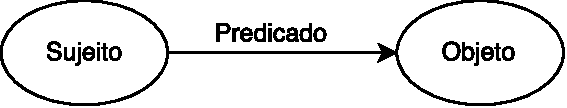
\includegraphics[width=0.5\textwidth]{./imagens/Sujeito-predicado-objeto.pdf}
    \caption{Estrutura da tripla RDF}
%	\footnotesize{Fonte: Próprio autor.}
	\label{fig:spo}
\end{figure}

A estrutura do RDF pode se materializar de várias formas. Cada uma dessas formas recebe o nome de serialização RDF. Atualmente existe um conjunto considerável de serializações tais como: RDF/XML, Turtle, N-Triples e outros. Onde cada serialização tem um uso em potencial. Por exemplo, Turtle é usado para ser lido por humanos, pois ele é melhor estruturado para isso. 

Vale a pena salientar que RDF é um framework de descrição, não sendo responsável por atribuir semântica aos recursos descritos, sendo as ontologias responsáveis por esta função. Por esta razão, um número considerável de processos de publicação de Dados Conectados \cite{bizer2007publish, hyland2011joy, villazon2011methodological, Avila2015} recomenda o reuso de ontologias. 

\section{Ontologias}
Os Dados Conectados fazem uso de ontologias como suporte formal para representação de conhecimento, pois só RDF não é o bastante para que máquinas consigam entender a relação entre os dados. Desta forma, as ontologias têm um papel fundamental na modelagem e descrição de dados. A palavra ontologia vem do Grego \textit{ontos} e \textit{logos}, significando conhecimento do ser. Em filosofia, ontologia refere-se ao estudo do ser. Em Computação, de maneira informal, uma ontologia define um conjunto de conceitos e suas relações, tais como a terminologia (vocabulário do domínio), definição explícita dos conceitos essenciais, suas classificações, taxonomias, relações e axiomas do domínio, incluindo hierarquias e restrições \cite{deved2006semantic}. Em 1993, \citeauthor{gruber1993translation} definiu ontologia como uma especificação explícita de uma conceitualização. Em 1997, \citeauthor{borstw1997construction} definiu ontologia como uma especificação formal de uma conceitualização compartilhada. Em 1998, \citeauthor{studer1998knowledge} unificaram as duas definições, desta forma ontologia pode ser definida como uma especificação formal e explícita de uma conceitualização compartilhada. Para melhor entendimento, abaixo seguem detalhes sobre os termos citados nessa definição: 
% * <profsean@gmail.com> 2017-01-18T19:49:08.414Z:
% 
% > \citeauthor{studer1998knowledge}
% Aqui o formato da citação está errado... Não entendi o motivo...
% 
% ^ <armandobs14@gmail.com> 2017-01-18T20:06:42.666Z:
%
% Isso ocorre por erro no bibtex, estou ajustando.
%
% ^ <armandobs14@gmail.com> 2017-01-18T20:06:50.399Z.
\begin{itemize}
	\item \textbf{Explícita:} definições de conceitos, relações, restrições e axiomas; 
	\item \textbf{Formal:} compreensível para agentes e sistemas; 
	\item \textbf{Conceitualização:} modelo abstrato de uma área de conhecimento; 
	\item \textbf{Compartilhada:} conhecimento consensual. 
\end{itemize}
Pode-se concluir, a partir das características supracitadas sobre ontologias, que o conhecimento é explícito. Esse conhecimento equivale à descrição de determinada área do conhecimento, garantindo um conhecimento “consensual” sobre tal área. A partir do momento em que há um consenso, há a possibilidade e a viabilidade de compartilhar tais ontologias e integrá-las a outras áreas de conhecimento (através de outras ontologias).

\section{Dados Conectados}
O termo Dados Conectados (do inglês Linked Data) é a tradução oficial para o conceito na língua portuguesa \cite{Isotani2015}. Segundo o W3C, Dados Conectados pode ser entendido como o núcleo da Web Semântica, tendo como objetivo prover a integração e raciocínio de dados disponíveis na Web. Além disso, \citeonline{berners2006linked} ressalta que Dados Conectados não se trata apenas de pôr dados na internet, mas fazer conexões entre eles, permitindo que pessoas ou máquinas possam explorar a Web dos dados.

Para conectar os dados disponíveis na Web com qualidade, foram desenvolvidas as boas práticas. Essas boas práticas são fundamentadas em tecnologias Web como ressaltam \citeonline{Isotani2015}. Além dessas tecnologias, vale a pena destacar os quatro princípios básicos de Dados Conectados \cite{berners2006linked}: 

\begin{enumerate}
	\item Usar URI para a identificação de recursos
	\item Usar HTTP URIs para que seja possível buscar pelos recursos 
	\item Prover informação útil para as URIs consultadas através de padrões (RDF e SPARQL) 
	\item Incluir links para outras URIs. Possibilitando a descoberta de novos recursos
\end{enumerate}

É possível dividir os princípios em duas categorias. A primeira categoria é composta pelos dois primeiros princípios, estando relacionada a identificação e resolução desses recursos através de URI e HTTP URIs. A segunda categoria está relacionada de forma prática à conexão dos dados, utilizando RDF para especificar como os recursos são descritos e URIs que apontam para outros recursos, conectando de fato os dados.

\section{Algoritmos de similaridade}

Algoritmos de similaridade podem ser entendidos como funções utilizadas para medir a semelhança entre duas palavras. Tais funções são utilizadas em vários contextos, partindo de correções ortográficas até tarefas de processamento de linguagem natural (PLN). Um dos algoritmos de similaridade mais conhecidos pela comunidade foi proposto por Levenshtein em 1965 \cite{levenshtein1966binary}, que se baseia na quantidade mínima de edições (remoções e adições) necessárias para que uma palavra seja igual a outra.  

Dependendo da perspectiva dada ao texto (conjunto de caracteres e conjuntos de palavras) existem diferentes abordagens (baseadas em caractere, baseadas em \textit{token}) \cite{cohen2003comparison}. Abordagens baseadas em caractere (e.g. Levenshtein) realizam a comparação letra por letra. Já as abordagens baseadas em \textit{tokens} (e.g. Jaro) consideram a palavra como um corpo único.

Nesta proposta, foi utilizada uma generalização do algoritmo de Monge-Elkan \cite{monge1996field}, que tem o objetivo de dar um peso maior a \textit{tokens} mais semelhantes. Inicialmente, Monge-Elkan foi desenvolvido com o objetivo de calcular a semelhança entre textos que possuem vários \textit{tokens}, onde a similaridade de cada \textit{token} é calculada através da média das similaridades internas, que é provida por uma técnica baseada em caractere (e.g. Cosseno, Jaro, Dice). Essa abordagem se destaca em cenários de desordem ou ausência de \textit{tokens}. Além disso, esse algoritmo explora os benefícios providos pelas abordagens baseadas caractere (e.g. erros de digitação, erros de OCR e erros ortográficos) \cite{jimenez2009generalized}.

\section{Alinhamento de Dados Conectados}

Alinhar Dados Conectados  trata-se de um processo que tem como objetivo identificar e mesclar recursos que representam a mesma entidade do mundo real. Segundo \citeonline{homoceanu2014putting}, no contexto de dados conectados temos a seguinte definição para o problema:

\begin{equation}
f\left( { URI }_{ i },{ URI }_{ j } \right) :=\begin{cases} \mbox{verdadeiro, se } sim\left( { URI }_{ i },{ URI }_{ j } \right) >\theta  \\ \mbox{falso, caso contrário} \end{cases}\mbox{com }{ URI }_{ i } \in { D }_{ i }\mbox{ e }{ URI }_{ j } \in { D }_{ j }
\end{equation}

onde 1 $\leq$ i,j $\leq$ n, e $sim()$ é uma função que é capaz de calcular a similaridade entre os recursos e $\theta$ é o parâmetro que regula o nível de qualidade para o alinhamento, que também pode ser conhecido como limiar ou \textit{threshold}. Além disso, é possível ressaltar outros benefícios que surgem a partir da conexão entre dados, sendo elas: 

\begin{itemize}
	\item \textbf{Integração semântica de dados:} Refere-se ao melhoramento das técnicas existentes para descobertas de mapeamento (semi) automático entre ontologias heterogêneas e distribuídas; 
	\item \textbf{Reconhecimento de identidade:} Refere-se à capacidade de identificar se descritores de recursos distintos estão relacionados à mesma entidade do mundo real; 
	\item\textbf{ População de ontologias:} Refere-se à descoberta de relacionamentos entre novas instâncias e as instâncias já existentes na base de conhecimento. 
\end{itemize}

Segundo \citeonline{ferrara2008towards}, para que uma abordagem seja capaz de identificar recursos que identifiquem a mesma entidade do mundo real com propriedade essa deve satisfazer diferentes requisitos, que estão  dispostos em três categorias (ver Figura \ref{fig:imrequirements}).

\begin{figure}[!ht]
	\centering
%	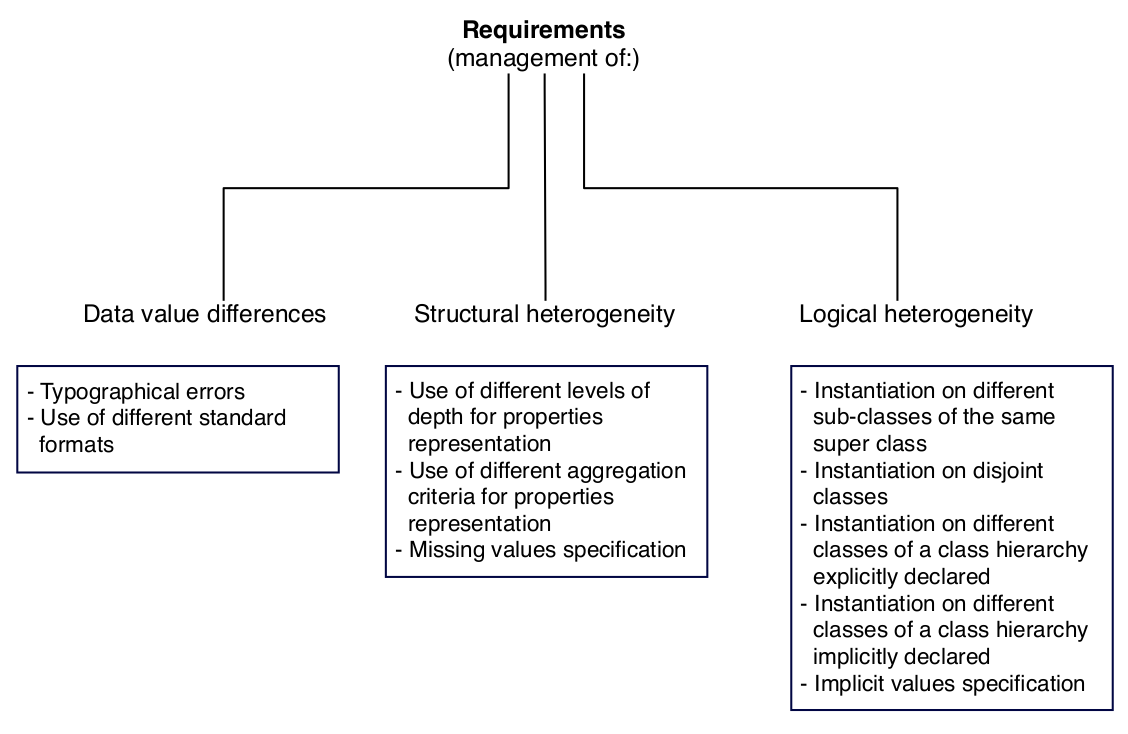
\includegraphics[width=0.9\textwidth]{./imagens/IMRequirements.png}
	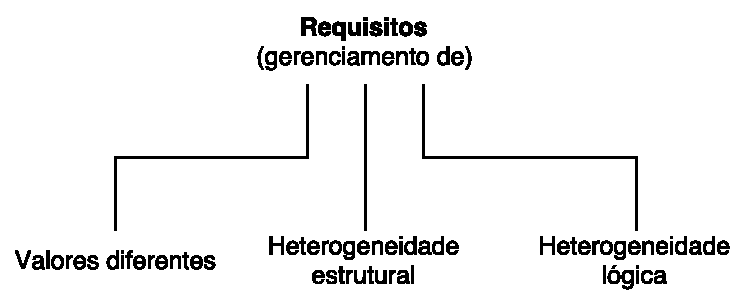
\includegraphics[width=0.9\textwidth]{./imagens/im_requirements.pdf}
    \caption{Requisitos para soluções de alinhamento de dados}
	\footnotesize{Fonte: baseado em \cite{ferrara2008towards}}
	\label{fig:imrequirements}
\end{figure}

\textbf{Valores diferentes:}
% * <profsean@gmail.com> 2017-01-18T20:15:13.295Z:
% 
% > Diferença de Valores:
% "Diferença de valores" (como está no texto) ou "Valores diferentes" (como está na figura)?
% 
% ^ <armandobs14@gmail.com> 2017-01-18T20:17:47.903Z:
%
% Ajustei para deixar de acordo com a imagem.
%
% ^ <armandobs14@gmail.com> 2017-01-18T20:17:50.727Z.
Um algoritmo de correspondência de instância deve reconhecer valores correspondentes, sempre que possível, mesmo quando esses valores possuem erros. Para mitigar esse problema, a comunidade utiliza abordagens como algoritmos de similaridade e transformação de valores.


\textbf{Heterogeneidade Estrutural:}
Instâncias que pertencem a ontologias diferentes diferem não somente entre propriedades e valores, mas também na sua estrutura. Desta forma, algoritmos de alinhamento de dados devem identificar propriedades semelhantes em ambos os recursos.


\textbf{Heterogeneidade Lógica:}
% * <profsean@gmail.com> 2017-01-18T20:18:47.062Z:
% 
% > Heterogeneidade Lógica:
% Não explicou...
% 
% ^ <armandobs14@gmail.com> 2017-01-18T20:36:14.777Z:
%
% O autor não descreve o que seria de fato a heterogeneidade lógica, dessa forma descrevi de acordo o meu entendimento.
%
% ^ <armandobs14@gmail.com> 2017-01-18T20:36:21.108Z.
A heterogeneidade lógica trata-se de um problema de alinhamento de ontologias, o qual não é levado em consideração no processo de alinhamento de dados, no entanto, faz-se necessário em tarefas de inferência. Esse problema diz respeito à semântica atribuída aos termos, havendo situações em que o mesmo termo pode ter significados diferentes atribuídos a ele (\textit{e.g.} manga - fruta e manga - vestimenta).

Diante do exposto, a comunidade vem desenvolvendo alternativas para a aperfeiçoar as soluções para a correspondência de instâncias 
